\section{Dirac Field Theory III}
We've written down the Lagrangian density for the Dirac field theory:
\begin{equation}
    \L = -i\bar{\psi}(\dirac + m)\psi
\end{equation}
where $\bar{\psi} = \psi^\dag \gamma^0$. We are discussing fermions, so the above Lagrangian concerns anti-commuting classical fields. Last time we discussed the Lorentz invariance of the Dirac Field Theory; now we can use Noether's theorem to find the conserved Noether current.

Before that; a quick question; why do we want a $-i$ there? Because $(\gamma^0)^2 = -1$ and therefore with the $-i$ we get the desired $i\psi^\dag \dpd{}{t}\psi$ term when expanding. It isn't a huge problem if we get the normalization wrong, but we've chosen the canonical normalization here.

Additionally, in the textbook, the derivative has been symmetrized. In the above form, the derivative only acts on the right. In the textbook, there is a $\stackrel{\leftrightarrow}{\dirac} = \stackrel{\rightarrow}{\dirac} - \stackrel{\leftarrow}{\dirac}$ in the Lagrangian due to the symmetrization.

Let's go ahead and analyze the symmetries of this theory. The most important one will not be the space-time translation symmetry, but rather the symmetry under phase transformations.

\subsection{Phase Symmetry}
We consider a variation of the fields:
\begin{equation}
    \delta \psi = i\psi, \quad \delta \bar{\psi} = -i\bar{\psi}
\end{equation}
It is easy to see that the Lagrangian is invariant under this phase transformation:
\begin{equation}
    \L = -i\bar{\psi}(\dirac + m)\psi \mapsto -i(-i\bar{\psi})(\dirac + m)(i\psi) = -i\bar{\psi}(\dirac + m)\psi = \L
\end{equation}
and so $\delta \L = 0$. Noether's theorem tells us that there is a conserved current:
\begin{equation}
    \mathcal{J}^\mu = \delta \psi \dpd{\L}{(\p_\mu \psi)} + \delta \bar{\psi}\dpd{\L}{(\p_\mu \bar{\psi})} = \bar{\psi}\gamma^\mu \psi
\end{equation}
And therefore:
\begin{equation}
    \p_\mu \mathcal{J}^\mu = \p_\mu\left(\bar{\psi}\gamma^\mu \psi\right) = 0.
\end{equation}
Let's give this an overall factor of minus one for notational consistency (so when we have $(\gamma^0)^2 = -1$ the minus sign cancells):
\begin{equation}
    \mathcal{J}^\mu(x) = -\bar{\psi}\gamma^\mu \psi
\end{equation}
and so much like the previous case, we have the conservation of particle number due to phase symmetry.

\subsection{Spacetime Symmetry}
One of these symmetries is just translations:
\begin{equation}
    \delta_{(\mu)}\psi = -\p_\mu \psi
\end{equation}
Then:
\begin{equation}
    \delta_{(\mu)}\L = -\p_\mu \L
\end{equation}
as there is no explicit coordinate dependence in the Lagrangian density. So, this is a symmetry and so we can write:
\begin{equation}
    \mathcal{J}_{(\mu)}^\nu(x) = \delta_{(\mu)}\psi \dpd{\L}{(\p_\nu \psi)} + \delta_{(\mu)} \bar{\psi}\dpd{\L}{(\p_\nu\bar{\psi})} + \eta^{\nu}_\mu \L(x).
\end{equation}
The second term is zero as there is no $\p_\nu \bar{\psi}$ dependence in the Lagrangian density. The first term we can easily read off, so the above evauates to:
\begin{equation}
    \mathcal{J}_{(\mu)}^\nu(x) = -i\bar{\psi}\gamma^\mu \p_\mu \psi - i\eta^{\mu}_\nu \bar{\psi}(\dirac + m)\psi.
\end{equation}
Since we've now derived the conserved current (independent of the equation of motion), we are now free to rewrite it in a cleaner form using the EoM. Doing so, we can eliminate the last term. We can then write the above as:
\begin{equation}
    \mathcal{J}_{(\mu)}^\nu(x) = \mathbb{T}_{0\mu}^{\nu}(x)
\end{equation}
Then:
\begin{equation}
    \p_\nu \mathbb{T}^\nu_{0\mu} = i\bar{\psi}\dirac \p_\mu \psi + i\bar{\psi}\stackrel{\leftarrow}{\dirac}\p_\mu \psi
\end{equation}
The EoM tells us:
\begin{equation}
    (\dirac + m)\psi = 0, \quad \psi^\dag\left(\stackrel{\leftarrow}{\dirac} + m\right) = 0.
\end{equation}
and multiplying on the right by $\gamma^0$:
\begin{equation}
    \bar{\psi}\left(-\stackrel{\leftarrow}{\dirac} + m\right) = 0
\end{equation}
and hence:
\begin{equation}
    \p_\nu \mathbb{T}^\nu_{0\mu} = i\bar{\psi}\dirac \p_\mu \psi + i\bar{\psi}\stackrel{\leftarrow}{\dirac}\p_\mu \psi = 0.
\end{equation}

It's worth pointing out that this stress tensor seems problematic off the bat; it's not symmetric. This turns out to be not a problem, though.

\subsection{Lorentz Symmetry}
The infinitesimal Lorentz transformation of the fields reads:L
\begin{equation}
    \delta \psi = \omega_{\mu\nu}\left((x^\mu \p^\nu - x^\nu \p_\mu)\psi - \frac{1}{4}[\gamma^\mu, \gamma^\nu]\right)\psi
\end{equation}
note that $[\gamma^\mu, \gamma^\nu]$ is often called the spin tensor.

We're going to take a bit of a simplifying shortcut to proceed. We can plug this into the Lagrangian density, and we will find that:
\begin{equation}
    \delta \L = \omega_{\mu\nu}(x^\mu \p^\nu - x^\nu \p^\mu)\L(x)
\end{equation}
which doesn't look like a symmetry, but by the antisymmetry of $\omega$ we can exchange the order of the derivative and hence the above becomes something like $\delta \L = \p(\ldots)$ and so is a symmetry. We find the conserved Noether current to be:
\begin{equation}
    \mathcal{J}^\lambda (x) = (x^\nu \mathbb{T}_0^{\lambda\mu} - x^\mu \mathbb{T}_0^{\lambda \nu})\omega_{\mu\nu} - \frac{i}{4}\bar{\psi}[\gamma^\lambda, [\gamma^\mu, \gamma^\nu]]\psi \omega_{\mu\nu}.
\end{equation}
We then have:
\begin{equation}
    0 = \p_\lambda \mathcal{J}^\lambda = (\mathbb{T}_0^{\nu\mu} - \mathbb{T}_0^{\mu\nu})\omega_{\mu\nu} + \omega_{\mu\nu}\p_\lambda\left(\frac{i}{4}\bar{\psi}[\gamma^\lambda, [\gamma^\mu, \gamma^\nu]]\psi\right)
\end{equation}
the above identity could be proven using algebra, but let's just rely on Noether's theorem to save us the Hassle. However, the above identity does give us something nice; it allows us to improve the stress tensor, symmetrizing it:
\begin{equation}
    \mathbb{T}^{\mu\nu}(x) = \frac{i}{2}\bar{\psi}\left(\gamma^\mu \p^\nu + \gamma^\nu \p^\mu\right)\psi
\end{equation}
%Note the bracket $[\gamma^\lambda, [\gamma^\mu, \gamma^\nu]]$ is antisymmetric in the indices and hence taking further derivatives will result in zero
If we contract the above with a Killing vector, we find:
\begin{equation}
    \mathcal{J}^{\lambda}_f = \mathbb{T}^{\mu\nu}\hat{f}_\nu(x).
\end{equation}
What is more, if the fermion is massless, the $\mathbb{T}^{\mu\nu}$ has vanishing trace! This is because when we take the trace, $\gamma^\mu\p^\nu$ turns into a $\dirac$. Therefore $\mathbb{T}^{\mu\nu}\hat{f}_\nu(x)$ is a conserved current even if $\hat{f}$ is not a Killing vector but a conformal Killing vector.

If we look at the Hamiltonian here, we get the (matrix-valued) Dirac Hamiltonian which we have to confirm is actually sensible. This will have negative and positive eigenvalues. If we chose bosons instead of fermions, it would not be bounded from below; as bosons will arbitrarily fill the negative energy states. We have the so called ``Dirac sea'', which is stabilized in the case of Fermions (as it is totally filled), like the case of the Fermi sea. Note that in constrast to the Fermi sea however, we have an infinitely deep sea! Another contrast; in the Fermi gas system we have a metal, while in the Dirac field system we have an insulator as there is an energy gap between the dirac sea (negative energy states) and the positive energy states.

\begin{figure}[htbp]
    \centering
    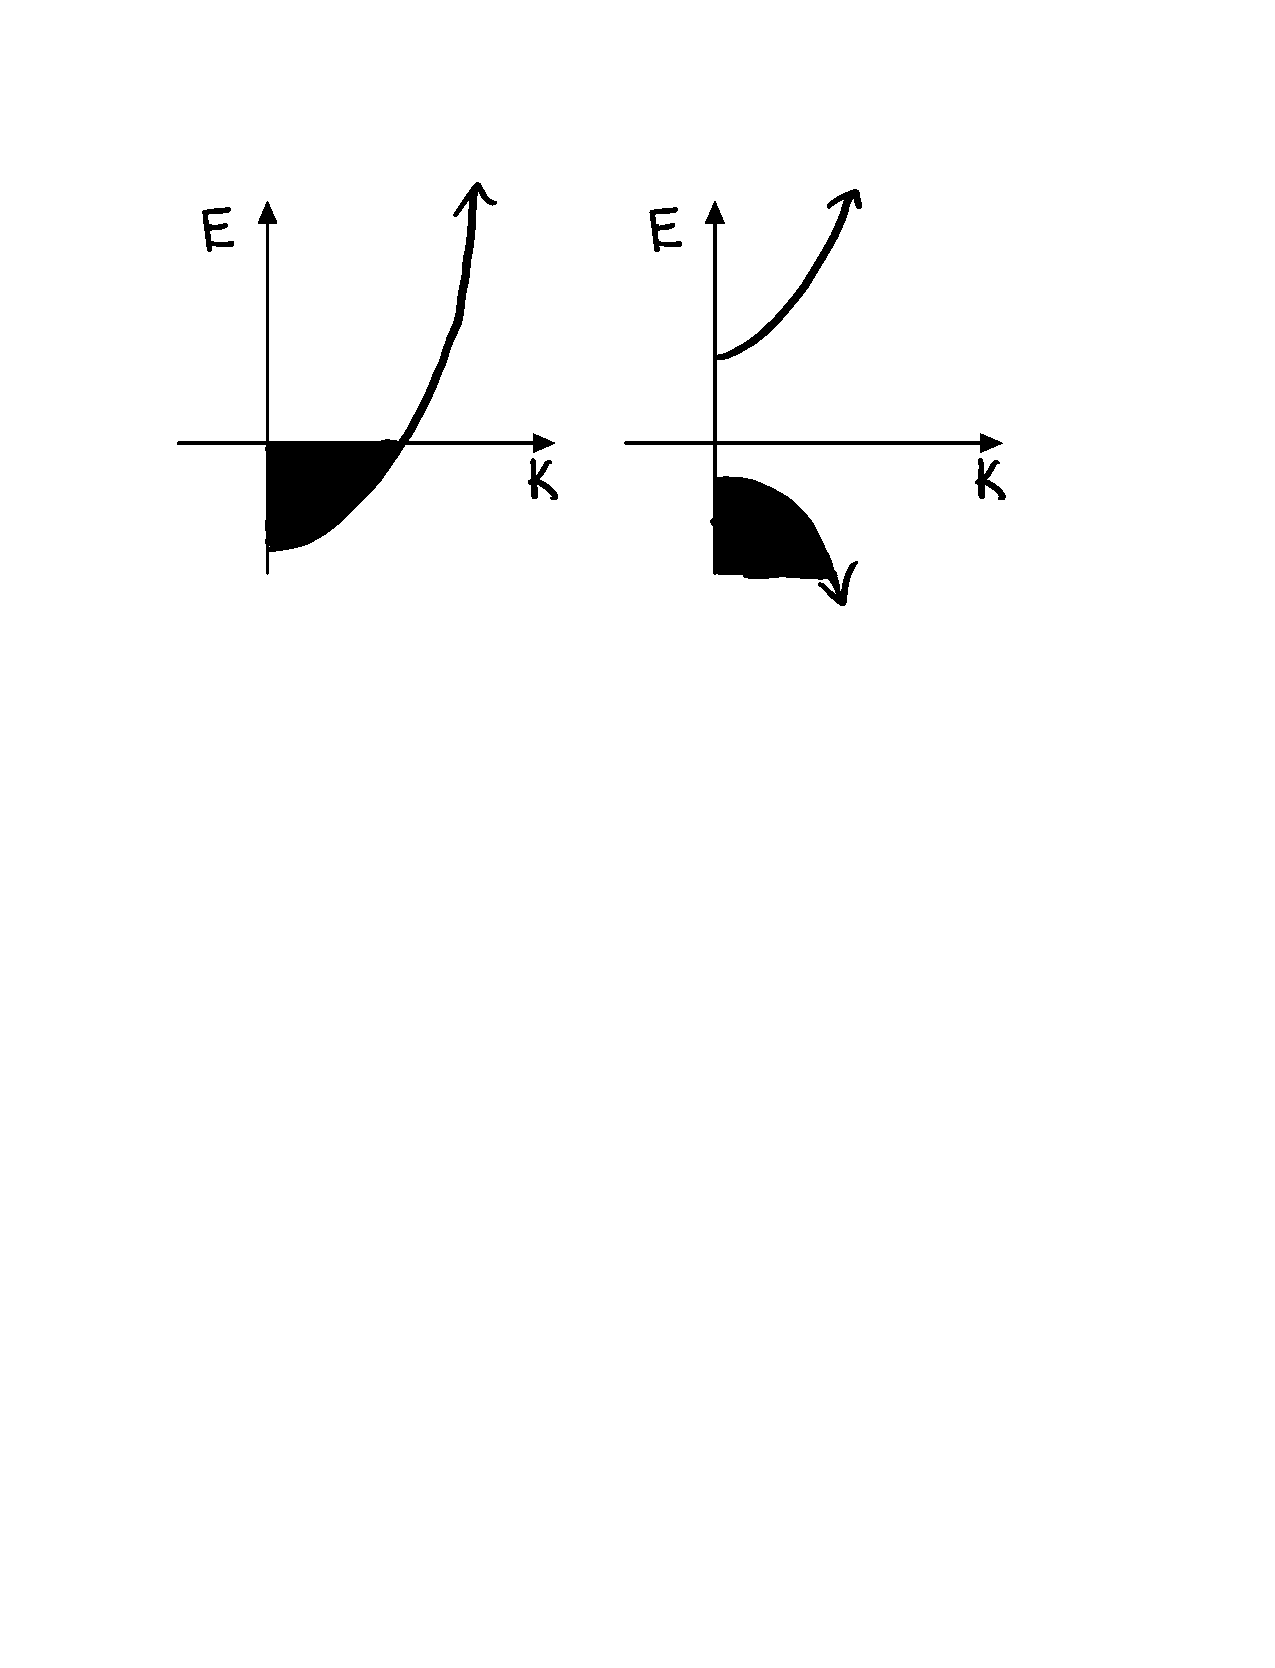
\includegraphics[scale=0.7]{Images/fig-fermidiracseas.pdf}
    \caption{Sketch of the energies of a degenerate Fermi gas (left) and the Dirac field (right). The shaded region corresponds to the Fermi and Dirac ``seas'', respectively.}
    \label{fig-fermidiracseas}
\end{figure}

The infinitely deep quality of the Dirac sea has some interesting implications. It gives us a way to violate some symmetries, for example, e.g. the symmetry that shifts all levels by a unit. In the dirac sea case, if we moved up one unit we would create a particle in the positive energy region and if we moved down unit we would create a hole in the negative energy region.


\subsection{Starting to Solve the Dirac Equation}
So, we've pretty comprehensively studied the symmetries of the Dirac theory. The last thing left is to actually solve it. We consider the representation:
\begin{equation}
    \gamma^0 = \m{0 & \mathbb{I} \\ -\mathbb{I} & 0}, \quad \gamma^a = \m{0 & \sigma^a \\ \sigma^a & 0}
\end{equation}
where $\sigma^a$ are the Pauli matrices:
\begin{equation}
    \sigma^1 = \paulix, \quad \sigma^2 = \pauliy, \quad \sigma^3 = \pauliz
\end{equation}
We then have that rotations in the $ab$ plane (about the $c$ axis) looks like:
\begin{equation}
    \frac{i}{4}[\gamma^a, \gamma^b] = -\e^{abc}\m{\frac{\sigma^c}{2} & 0 \\ 0 & \frac{\sigma^c}{2}}
\end{equation}
where the commutators are easily computed using the Pauli algebra. This is a nice representation as the spins are indeed actual spins/rotations, in a sense. 

We consider a four-spinor plane wave ansatz:
\begin{equation}
    \psi(x) = \m{u \\ v}e^{i\left(\v{k}\cdot\v{x} - \omega(\v{k})t\right)}
\end{equation}
In the chosen matrix representation, the Dirac equation with the above ansatz becomes:
\begin{equation}
    \m{m & i\omega + i\gv{\sigma} \cdot \v{k} \\ -i\omega + i\gv{\sigma} \cdot \v{k} & m}\m{u\\v} = 0.
\end{equation}
and so if we solve the eigenvalues and eigenvectors of the above, we are done! We can see that the spin plays a very active role here due to the $\gv{\sigma}\cdot \v{k}$ (spin-momentum coupling). We can see that spin is not a good quantum number here as the spin rotation messes it up. What is a good quantum number is if we look for the eigenvalues of $\gv{\sigma} \cdot \v{k}$ - this is related to the spin along the direction of motion of the particle, or the \emph{helicity}. We will discuss it more next time, where we will conclude our discussion of the Dirac field. We will then move onto photons!